\documentclass[border=10pt]{standalone}
\usepackage{pgfplots}
\usepgfplotslibrary{colormaps}
\pgfplotsset{compat=1.18}

\begin{document}
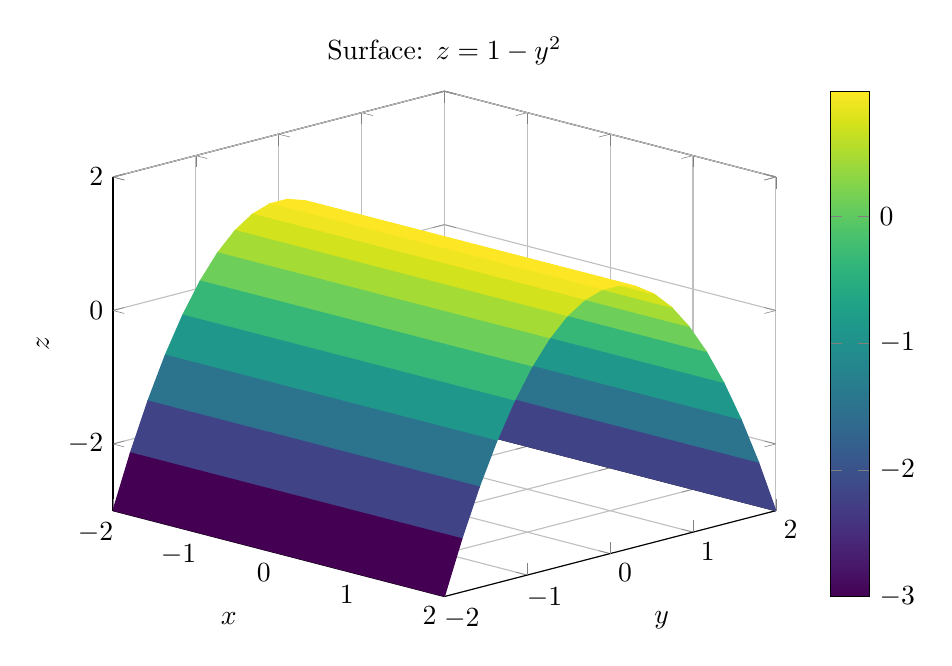
\begin{tikzpicture}
\begin{axis}[
    view={45}{20},
    xlabel={$x$},
    ylabel={$y$},
    zlabel={$z$},
    title={Surface: $z = 1 - y^2$},
    domain=-2:2,
    y domain=-2:2,
    samples=20,
    samples y=20,
    colormap/viridis,
    colorbar,
    grid=major,
    width=10cm,
    height=8cm,
    zmin=-3,
    zmax=2
]
\addplot3[surf, shader=flat corner] {1 - y^2};
\end{axis}
\end{tikzpicture}
\end{document}